\section{Background}\label{sec:background}

The dataset to be used is a set of neuro-imaging scans from a cohort of 30 healthy, young women in the
Netherlands circa 2013 who were presented with various grids of images featuring
either neutral entities, (e.g.\ office chairs, windows, jackets) or foods~\cite{smeets2013allured}.
The foods were specifically types of calorically dense, tempting foods, which the individuals viewing would likely
have formed restraint with given their success in maintaining healthy body mass indices.
The experiment was meant to highlight brain structures roles in anticipated rewards from consuming delicious foods,
balanced against the hypothesized activation of restraints.

In neuro-imaging, this task is known as passive image viewing.

Given the quite important role of food and willpower in our lives, the activation patterns are likely to be powerful
and distinguishable from neutral objects which we haven't evolved to be nearly as concerned with.
This combination makes this an excellent selection for a proof of concept application of deep learning as the chances
of success on a less subtle activation pattern, observable to trained researchers, are quite high.
This specific application then can serve as a jumping off point for future works where the activity patterns are less
distinguishable, and may be an interesting addition to the works in brain-pattern controlled prosthetics.
This dataset is also ideal as it comes with a fairly usable ground-truth labeling mechanism, as I am not currently
investigating the capacity for unsupervised differentiation.

\subsection{Data Format}\label{subsec:data-format}

The dataset can be found from the excellent
OpenNeuro project here: \url{https://openneuro.org/datasets/ds000157/versions/00001}

The dataset follows the BIDS (Brain Imaging Data Structure) layout adopted by many neuroscience researchers.
It consists of a survey detailing the relationship of each of the 30 subjects with food and diet taken after the experimental
proceedings, and the core data of two modalities of brain imaging: a single high resolution T1w Modality fMRI scan seen in figure~\ref{fig:ortho-t1w},
and time series of 370-375 BOLD Modality fMRI scans seen in figure~\ref{fig:ortho-bold}, encompassing approximately 10 minutes
capturing brain activity of the subjects during their exposure to the experimental triggers.

The bold scans are quite sizeable as far as datasets go, given the number of each per subject,
however they are a relatively low resolution, consisting
of 64 sagital by 64 coronal by 30 axial scans, with only a single image channel.

The activation is measured in a positive magnitude visible in figure~\ref{fig:ex_stat_map}, through a helper method in a neuro-imaging specialized
image handling library ~\cite{brett_matthew_2019_3544468}.

I had to manually infer pairings of the scans with the experimental phase for classification training given the events log associated
with each subject and the advertised scan times from the paper.
While the data does appear healthy, there may be some discrepancies of interpretation which would warrant future investigation if the
performance on this particular experiment was the primary focus.


 \begin{figure}
  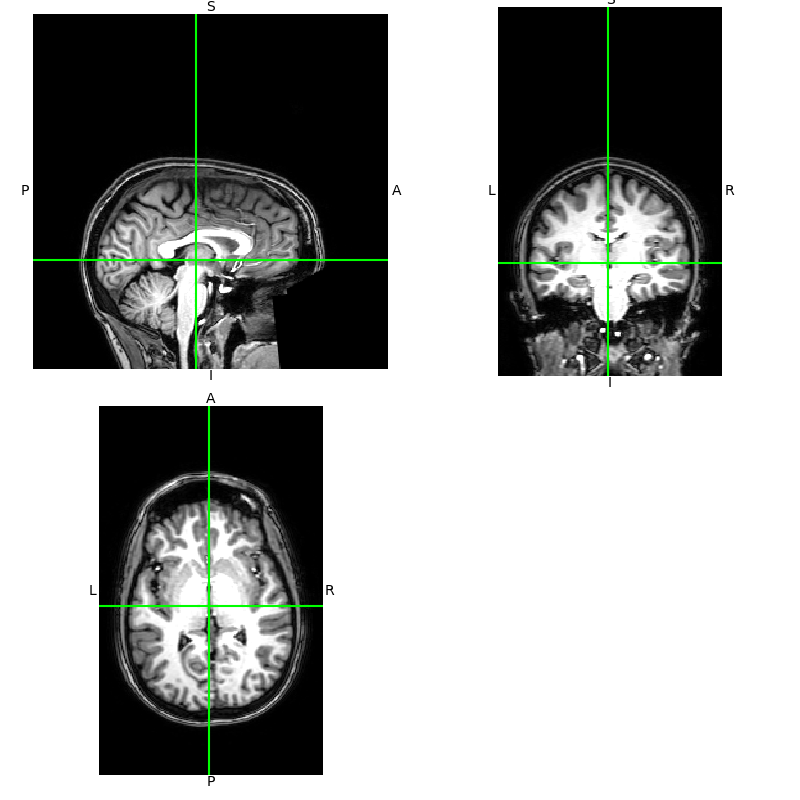
\includegraphics[width=\linewidth]{images/orthoview_t1w.png}
  \caption{T1w Modality High-Res 3d Scan of Subject Brain}
  \label{fig:ortho-t1w}
\end{figure}

\begin{figure}
  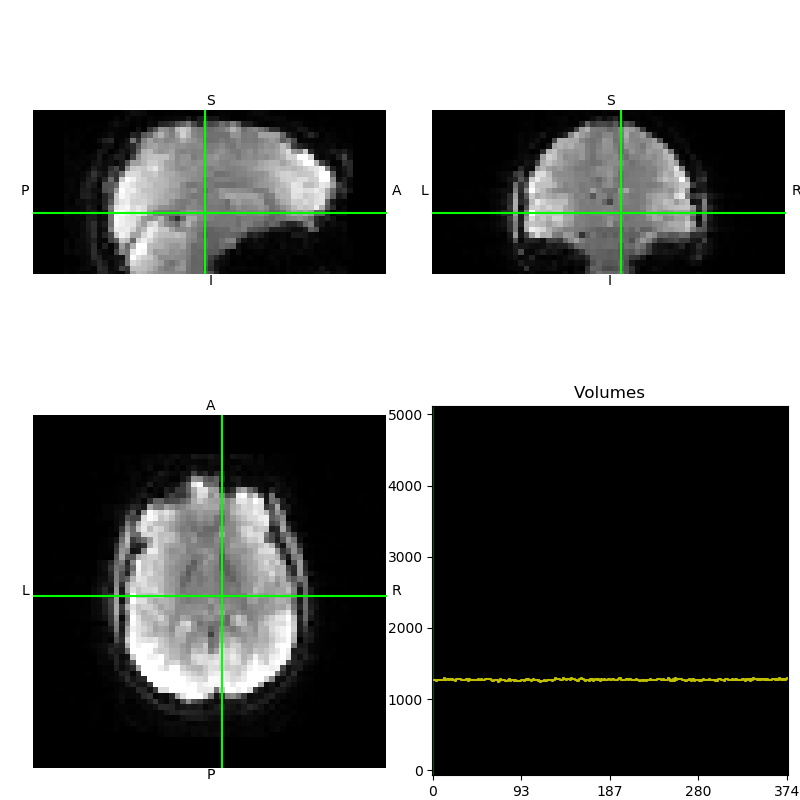
\includegraphics[width=\linewidth]{images/orthoview_bold.png}
  \caption{Bold Modality Low-Res 3d Experimental Scans of Subject Brain}
  \label{fig:ortho-bold}
\end{figure}

\begin{figure}
  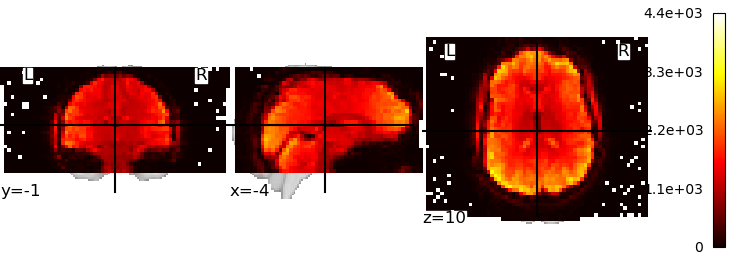
\includegraphics[width=\linewidth]{images/example_stat_map.png}
  \caption{Activity Measures from Bold Scans}
  \label{fig:ex_stat_map}
\end{figure}

\subsection{Review}\label{subsec:review}

You may review the full experimental paper as well here: \url{http://www.pamitc.org/documents/mermin.pdf}.

You may find this project repository here: (personal github link removed for anonymity)
Reading the paper is critical to understanding the format of the dataset, however I hope I will provide enough
abstraction in the project repository for you to be freed of that challenge should you wish to have a look around.
